\documentclass[a4paper,oneside,DIV=12,12pt,headings=normal]{scrartcl}

%%% Length calculations
\usepackage{calc}
%%%

%%% Support for color
\usepackage{xcolor}
\definecolor{lightblue}{HTML}{03A9F4}
\definecolor{red}{HTML}{F44336}
%%%

%%% Graphics inclusion
\usepackage{graphicx}
%%%

%%% Font selection
\usepackage{fontspec}

\setromanfont{STIX Two Text}[
	SmallCapsFeatures = {LetterSpace = 5},
]

\setsansfont{Source Sans Pro}[
]

\setmonofont{Source Code Pro}[
]
%%%

%%% Math settings
\usepackage{amsmath,unicode-math}
\setmathfont{STIX Two Math}

\usepackage{IEEEtrantools}
\usepackage{mleftright}
%%%

%%% Font settings for different KOMA Script elements
\setkomafont{pagenumber}{\rmfamily}
\setkomafont{disposition}{\rmfamily\bfseries}
%%%

%%% Typographic enhancements
\usepackage{microtype}
%%%

%%% Language-specific settings
\usepackage{polyglossia}
\setmainlanguage{ukrainian}
%%%

%%% List settings
\usepackage{enumitem}
\setlist[enumerate]{
	leftmargin = *,
}
%%%

%%% Captions
\usepackage{caption}
\usepackage{subcaption}

\DeclareCaptionLabelFormat{closing}{#2)}
\captionsetup[subtable]{labelformat = closing}
\captionsetup[subfigure]{labelformat = closing, position = auto}
%%%

%%% Tables
\usepackage{booktabs}
\usepackage{longtable}

\usepackage{multirow}

\usepackage{array}
\newcolumntype{v}[1]{>{\raggedright\arraybackslash\hspace{0pt}}p{#1}}
\newcolumntype{b}[1]{>{\centering\arraybackslash\hspace{0pt}}p{#1}}
\newcolumntype{n}[1]{>{\raggedleft\arraybackslash\hspace{0pt}}p{#1}}

\usepackage{kbordermatrix} % labeling array indices
%%%

%%% Floats on a single row
\usepackage{floatrow}
\newfloatcommand{capbtabbox}{table}[][\FBwidth]
%%%

%%% Links and hyperreferences
\usepackage{hyperref}
\hypersetup{
	colorlinks      = false,
	linkbordercolor = red,
	urlbordercolor  = lightblue,
	pdfborderstyle  = {/S/U/W 1.5},
}
%%%

%%% All caps
\newcommand{\allcaps}[1]{{\addfontfeatures{LetterSpace = 3}#1}}
%%%

\setlength{\emergencystretch}{1em}

\begin{document}
	\begin{titlepage}
	\centering
		Міністерство освіти і~науки України\\
		Національний авіаційний університет\\
		Навчально-науковий інститут комп'ютерних інформаційних технологій\\
		Кафедра комп'ютеризованих систем управління

		\vspace*{\fill}

		Лабораторна робота №4\\
		з дисципліни «Комп'ютерна схемотехніка»\\
		на тему «Дослідження суматорів»

		\vspace*{\fill}
		
		\begin{flushright}
			Виконав:\\
			студент ННІКІТ СП-225\\
			Клокун В.\,Д.\\
			Перевірив:\\
			Іскренко Ю.\,Ю.
		\end{flushright}

		Київ 2018
	\end{titlepage}

	\section{Мета роботи}
		Вивчення принципів побудови і~логіки роботи двійкових сумматорів \allcaps{ЕОМ}. Освоєння методики визначення статичних і~динамічних характеристик суматорів \allcaps{ЕОМ}. Ознайомлення з~суматорами \allcaps{ЕОМ} в~серіях інтегральних мікросхем~\allcaps{ТТЛШ}.

	\section{Хід роботи}
		\subsection{Дослідження схеми напівсуматора на логічних елементах І—НЕ}
			Перетворюємо рівняння напівсуматора до вигляду, зручного для реалізації на елементах І—НЕ:
			\begin{equation*}
				M_1 = \neg \left( \neg \left( \neg X_1 \land Y_1 \lor X_1 \land \neg Y_1 \right) \right)
				    = \neg \left( \neg X_1 \land Y_1 \land X_1 \land \neg Y_1 \right), \quad
				R_i = \neg \left( X_1 \land Y_1 \right).
			\end{equation*}
			На основі отриманих рівнянь складаємо схему напівсуматора на елементах І—НЕ~(рис.~\ref{fig:01-halfsum-schematic}). Підключаємо входи $X_1 X_1$ і~$Y_1 Y_1$ до тумблерного регістра, а~виходи $M_1$ і~$R_1$~— до світлових індикаторів. Досліджуємо роботу напівсуматора~(табл.~\ref{tab:01-halfsum-truth-table}). Задаємо значення вхідних змінних за допомогою тумблерів та~записуємо їх. Порівнюємо отримані результати з~теоретичними даними.

			\begin{figure}[!htbp]
				\begin{floatrow}
					\ffigbox[\FBwidth]{
						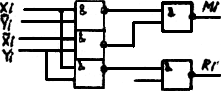
\includegraphics[width = 0.33\textwidth]{./assets/01.png}
					}{
						\caption{Схема напівсуматора на логічних елементах І—НЕ}
						\label{fig:01-halfsum-schematic}
					}
					\capbtabbox[\Xhsize]{
						\begin{tabular}{llrr}
							\toprule
								$X_1$ & $Y_1$ & $M_1$ & $R_1$ \\
							\midrule
								0     & 0     & 0     & 0 \\
								0     & 1     & 1     & 0 \\
								1     & 0     & 1     & 0 \\
								1     & 1     & 0     & 1 \\
							\bottomrule
						\end{tabular}
					}{
							\caption{Таблиця істинності напівсуматора на логічних елементах І—НЕ}
							\label{tab:01-halfsum-truth-table}
					}
				\end{floatrow}
			\end{figure}

		\subsection{Дослідження схеми напівсуматора на логічних елементах І—АБО—НЕ}
			Перетворюємо рівняння напівсуматора до вигляду, зручного для реалізації на елементах І—АБО—НЕ:
			\begin{IEEEeqnarray*}{rCl}
				M_1 &=& \neg X_1 \land Y_1 \lor X_1 \land \neg Y_1
				     =  \neg \left( X_1 \land Y_1 \lor \neg X_1 \land \neg Y_1 \right),\\
				R_i &=& \neg \left (\neg \left( X_1 \land Y_1 \right) \right)
				     =  \neg \left( \neg X_1 \lor \neg Y_1 \right).
			\end{IEEEeqnarray*}
			На основі отриманих рівнянь складаємо схему напівсуматора на елементах І—АБО—НЕ~(рис.~\ref{fig:02-halfsum-schematic}). Підключаємо входи $X_1 X_1$ і~$Y_1 Y_1$ до тумблерного регістра, а~виходи $M_1$ і~$R_1$~— до світлових індикаторів. Досліджуємо роботу напівсуматора~(табл.~\ref{tab:02-halfsum-truth-table}). Задаємо значення вхідних змінних за допомогою тумблерів та~записуємо їх. Порівнюємо отримані результати з~теоретичними даними.

			\begin{figure}[!htbp]
				\begin{floatrow}
					\ffigbox[\FBwidth]{
						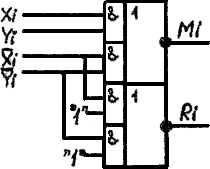
\includegraphics[width = 0.33\textwidth]{./assets/02.png}
					}{
						\caption{Схема напівсуматора на логічних елементах І—АБО—НЕ}
						\label{fig:02-halfsum-schematic}
					}
					\capbtabbox[\Xhsize]{
						\begin{tabular}{llrr}
							\toprule
								$X_1$ & $Y_1$ & $M_1$ & $R_1$ \\
							\midrule
								0     & 0     & 0     & 0 \\
								0     & 1     & 1     & 0 \\
								1     & 0     & 1     & 0 \\
								1     & 1     & 0     & 1 \\
							\bottomrule
						\end{tabular}
					}{
							\caption{Таблиця істинності напівсуматора на логічних елементах І—АБО—НЕ}
							\label{tab:02-halfsum-truth-table}
					}
				\end{floatrow}
			\end{figure}


		\subsection{Дослідження схеми однорозрядного суматора на логічних елементах І—НЕ}
			Перетворюємо рівняння однорозрядного суматора до вигляду, зручного для реалізації на елементах І—НЕ:
			\begin{IEEEeqnarray*}{rCl}
				M_1 &=& \neg \left( \neg \left( \neg X_1 \land \neg Y_1 \land Z_i \lor \neg X_i \land Y_i \land \neg Z_i \lor X_i \land \neg Y_i \land \neg Z_i \lor X_i \land Y_i \land Z_i \right) \right) \\
						&=& \neg \left( \neg \left( \neg X_i \land \neg Y_i \land Z_i \right) \land \neg \left( \neg X_i \land Y_i \land \neg Z_i \right) \land \neg \left( X_i \land \neg Y_i \land \neg Z_i\right) \land \neg \left( X_i \land Y_i \land Z_i\right) \right),\\
				P &=& \neg \left( \neg \left( X_1 \land Y_1 \lor X_1 \land Z_1 \lor Y_1 \land Z_1 \right) \right) \\
					&=& \neg \left( \neg \left( X_1 \land Y_1 \right) \land \neg \left(X_1 \land Z_1 \right) \land \neg \left( Y_1 \land Z_1 \right) \right).
			\end{IEEEeqnarray*}
			На основі отриманих рівнянь складаємо схему однорозрядного суматора на елементах І—НЕ~(рис.~\ref{fig:03-sum-schematic}). Підключаємо входи $X_1 X_1$, $Y_1 Y_1$ і~$Z_1 Z_1$ до тумблерного регістра, а~виходи $S_1$ і~$P_1$~— до світлових індикаторів. Досліджуємо роботу однорозрядного суматора~(табл.~\ref{tab:03-sum-truth-table}). Задаємо значення вхідних змінних за допомогою тумблерів та~записуємо їх. Порівнюємо отримані результати з~теоретичними даними.

			\begin{figure}[!htbp]
				\begin{floatrow}
					\ffigbox[\FBwidth]{
						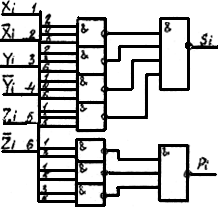
\includegraphics[width = 0.33\textwidth]{./assets/03.png}
					}{
						\caption{Схема однорозрядного суматора на логічних елементах І—НЕ}
						\label{fig:03-sum-schematic}
					}
					\capbtabbox[\Xhsize]{
						\begin{tabular}{lllrr}
							\toprule
								$X_1$ & $Y_1$ & $Z_1$ & $S_1$ & $P_1$\\
							\midrule
								0     & 0     & 0     & 0     & 0 \\
								0     & 0     & 1     & 1     & 0 \\
								0     & 1     & 0     & 1     & 0 \\
								0     & 1     & 1     & 0     & 1 \\
								1     & 0     & 0     & 1     & 0 \\
								1     & 0     & 1     & 0     & 1 \\
								1     & 1     & 0     & 0     & 1 \\
								1     & 1     & 1     & 1     & 1 \\
							\bottomrule
						\end{tabular}
					}{
							\caption{Таблиця істинності однорозрядного суматора на логічних елементах І—НЕ}
							\label{tab:03-sum-truth-table}
					}
				\end{floatrow}
			\end{figure}

		\subsection{Дослідження схеми однорозрядного суматора на логічних елементах І—АБО—НЕ}
			Перетворюємо рівняння однорозрядного суматора до вигляду, зручного для реалізації на елементах І—АБО—НЕ:
			\begin{IEEEeqnarray*}{rCl}
				S_i &=& \neg \left( \neg \left( X_i \land \neg P_i \lor Y_i \land \neg P_i \lor Z_i \land \neg P_i \lor X_i \land Y_i \land Z_i \right) \right), \\
				P_i &=& \neg \left( \neg \left( X_i \land Y_i \lor X_i \land Z_i \lor Y_i \land Z_i \right) \right).
			\end{IEEEeqnarray*}
			На основі отриманих рівнянь складаємо схему однорозрядного суматора на елементах І—АБО—НЕ~(рис.~\ref{fig:04-sum-schematic}). Підключаємо входи $X_1 X_1$, $Y_1 Y_1$ і~$Z_1 Z_1$ до тумблерного регістра, а~виходи $S_1$ і~$P_1$~— до світлових індикаторів. Досліджуємо роботу однорозрядного суматора~(табл.~\ref{tab:04-sum-truth-table}). Задаємо значення вхідних змінних за допомогою тумблерів та~записуємо їх. Порівнюємо отримані результати з~теоретичними даними.

			\begin{figure}[!htbp]
				\begin{floatrow}
					\ffigbox[\FBwidth]{
						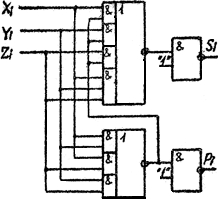
\includegraphics[width = 0.33\textwidth]{./assets/04.png}
					}{
						\caption{Схема однорозрядного суматора на логічних елементах І—АБО—НЕ}
						\label{fig:04-sum-schematic}
					}
					\capbtabbox[\Xhsize]{
						\begin{tabular}{lllrr}
							\toprule
								$X_1$ & $Y_1$ & $Z_1$ & $S_1$ & $P_1$\\
							\midrule
								0     & 0     & 0     & 0     & 0 \\
								0     & 0     & 1     & 1     & 0 \\
								0     & 1     & 0     & 1     & 0 \\
								0     & 1     & 1     & 0     & 1 \\
								1     & 0     & 0     & 1     & 0 \\
								1     & 0     & 1     & 0     & 1 \\
								1     & 1     & 0     & 0     & 1 \\
								1     & 1     & 1     & 1     & 1 \\
							\bottomrule
						\end{tabular}
					}{
							\caption{Таблиця істинності однорозрядного суматора на логічних елементах І—АБО—НЕ}
							\label{tab:04-sum-truth-table}
					}
				\end{floatrow}
			\end{figure}

	\section{Висновок}
		Під час виконання данох лабораторної роботи ми вивчили принципи побудови і~логіку роботи двійкових сумматорів \allcaps{ЕОМ}; освоїли методику визначення статичних і~динамічних характеристик суматорів \allcaps{ЕОМ}; ознайомились з~суматорами \allcaps{ЕОМ} в~серіях інтегральних мікросхем~\allcaps{ТТЛШ}.

\end{document}

